%& --translate-file=il2-pl
\documentclass[a4paper,12pt,final]{article}
\usepackage[left=2.5cm,right=2.5cm,bottom=2.5cm,top=2.5cm]{geometry}
\usepackage[american]{babel}
\usepackage[T1]{fontenc}
\usepackage[dvips]{graphicx}

%The new command form compound insertion definiton. That could be anything that you imagine.
\newcommand{\nrzw}[1]{{\Huge{\textbf{#1}}}}

\date{06/03/2005}

%opening
\title{The example article using konwerter}
\author{Piotr Wawrzyniak}

\begin{document}

\maketitle
\section{Preface}
In this document I persent some wonderful features of konwerter. If you see the source of this file, you will be able to more understand how this program works. The reaction.ps file, is the original file, with labels, that was not preprocessed by konwerter. Why it is ps file, not dvi? Because konwerter changes also eps files, and the dvi file strongly depends on it. It is just demonstration how all looks like before processing. Of course you can easily restore original format of eps files calling konwerter with -ntl option. The reaction.tex.auto.tex is the file, that was already processed. That file one should compile using latex, and after that one will get reaction.tex.auto.dvi file, that contains already not labels but numbers. The resultat that I've got one can see in the reaction.tex.auto.ps file. 

Before working one should create a special command form label inserting - $\backslash$nrzw\{\}. Here is what I did:
\begin{verbatim}
\newcommand{\nrzw}[1]{{\Huge{\textbf{#1}}}}
\end{verbatim}

I realized that it looks horrible, but it is just example. For konwerter it doesn't really matter what the new command does, so it can be anything.

To see how the konwerter works, please run it as follows:
\begin{verbatim}
konwerter reaction.tex 
latex reaction.tex.auto.tex
dvips -o reaction.tex.auto.ps
gv reaction.tex.auto.ps 
\end{verbatim}

The first command, converts all labels to numbers. As a~result you get the new reaction.tex.auto.tex file, that should be compiled with \LaTeX. The third command is the converting from dvi file to postscript, and the final command is seeing a~result.

Have a~great fun, using the konwerter.
\begin{flushright}
  Piotr Wawrzyniak
\end{flushright}

\newpage
\section{The acyloin condensation - arabic numbering.}
%We are including the eps file
%?plik{reaction.eps}
\begin{figure}[htp]
\includegraphics[width=1\textwidth]{reaction.eps}
\caption{The acyloin condensation mechanism.}
\end{figure}
Above we have the mechanism of the acyloin condensation. It is just great example of atak of the electron on the carbonyl group. The ester
 \nrzw{ester} is attacked by an electron, forming the anion radical \nrzw{radanion}. Two particles of \nrzw{radanion} can combine together,
  forming dianion \nrzw{dianion}, that after two OEt group removing forms diketon \nrzw{diket}. The next step of the reaction is once again attack of
   the electron and forming the compound \nrzw{rada}, that undergoes another electron attack, forming dianiondiradikal \nrzw{diadirad}. This
    particle can undergoes rearrangement to a compound \nrzw{dianion2}, that after protonation gives $\alpha$ hydroxyketon \nrzw{product}.
    
\newpage
\section{The acyloin condensation - roman numbering.}
\begin{center}
\textbf{We are starting numbering from 5: --set-r-to 5.}
\end{center}
%--set-r-to 5
%We are including the eps file
%?plik{reaction_roman.eps}
\begin{figure}[htp]
\includegraphics[width=1\textwidth]{reaction_roman.eps}
\caption{The acyloin condensation mechanism.}
\end{figure}
Above we have the mechanism of the acyloin condensation. It is just great example of atak of the electron on the carbonyl group. The ester
 \nrzw{:rester} is attacked by an electron, forming the anion radical \nrzw{:rradanion}. Two particles of \nrzw{:rradanion} can combine together,
  forming dianion \nrzw{:rdianion}, that after two OEt group removing forms diketon \nrzw{:rdiket}. The next step of the reaction is once again attack of
   the electron and forming the compound \nrzw{:rrada}, that undergoes another electron attack, forming dianiondiradikal \nrzw{:rdiadirad}. This
    particle can undergoes rearrangement to a compound \nrzw{:rdianion2}, that after protonation gives $\alpha$ hydroxyketon \nrzw{:rproduct}.

    \newpage
\section{The acyloin condensation - letters numbering.}
\begin{center}
\textbf{We are starting numbering from 10: --set-L-to 10.}
\end{center}
%--set-L-to 10
%We are including the eps file
%?plik{reaction_letters.eps}
\begin{figure}[htp]
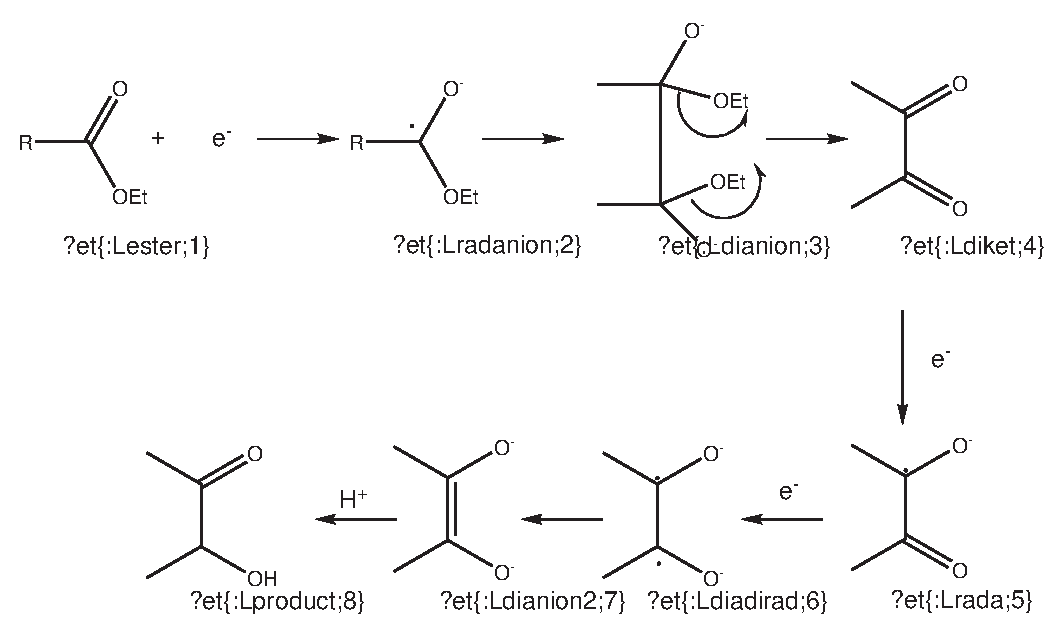
\includegraphics[width=1\textwidth]{reaction_letters.eps}
\caption{The acyloin condensation mechanism.}
\end{figure}
Above we have the mechanism of the acyloin condensation. It is just great example of atak of the electron on the carbonyl group. The ester
 \nrzw{:Lester} is attacked by an electron, forming the anion radical \nrzw{:Lradanion}. Two particles of \nrzw{:Lradanion} can combine together,
  forming dianion \nrzw{:Ldianion}, that after two OEt group removing forms diketon \nrzw{:Ldiket}. The next step of the reaction is once again attack of
   the electron and forming the compound \nrzw{:Lrada}, that undergoes another electron attack, forming dianiondiradikal \nrzw{:Ldiadirad}. This
    particle can undergoes rearrangement to a compound \nrzw{:Ldianion2}, that after protonation gives $\alpha$ hydroxyketon \nrzw{:Lproduct}.
\end{document}
